\documentclass[a4paper,12pt]{article}

\usepackage[utf8]{inputenc}
\usepackage[T1]{fontenc}
\usepackage{amsmath}
\usepackage{amssymb}
\usepackage{graphicx}
\usepackage{hyperref}
\usepackage{geometry}
\usepackage[italian]{babel}
\usepackage{svg}
\usepackage{float}
\usepackage{enumitem}

\geometry{a4paper, margin=1in}



\title{Progetto di Algoritmi e Protocolli per la Sicurezza}
\author{Davide D'Acunto\quad Noemi Biancamano}
\date{Gruppo 9}
\begin{document}

\maketitle

\tableofcontents
\newpage
\section{WP 1: Modello}
La seguente sezione si occupa di descrivere gli attori onesti presenti nel sistema, evidenziando le attività che sono interessati a svolgere.
\newline Successivamente, si procede alla discussione degli avversari e del threat model considerato, andando a specificare le capacità e le risorse da essi possedute. Infine, si presentano le proprietà che devono essere possedute dal sistema al fine di essere resiliente agli attacchi considerati.
\subsection{Attori \& Obiettivi}
\begin{figure}[H]
    \centering
    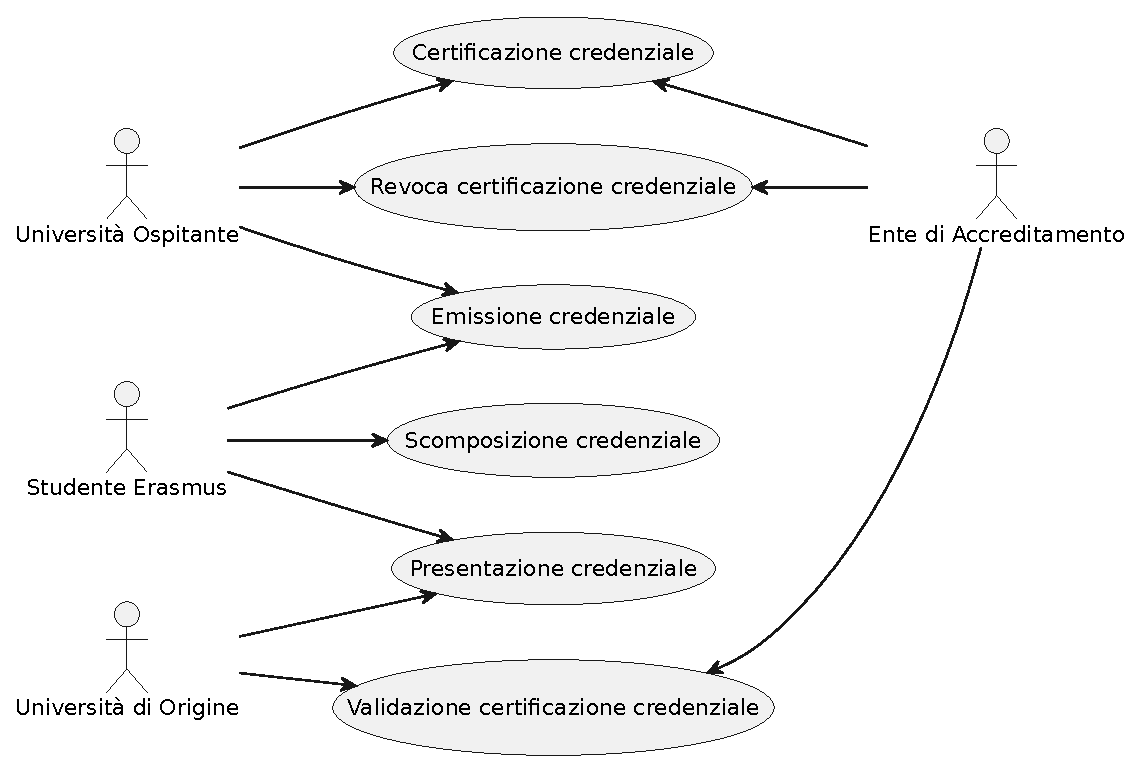
\includegraphics[width=0.95\textwidth]{usecase_1.eps}
    \caption{Use Case degli attori onesti}
    \label{fig:usecase1}
    
\end{figure}
\subsubsection{Studente Erasmus}
Lo studente Erasmus è interessato a sostenere attività accademiche all'interno della sede ospitante, le quali devono essere poi certificate e dimostrate all'università di origine.
\paragraph{Richiesta credenziale} Per cui lo studente necessita dall'università ospitante una credenziale accademica, che attesti le attività da egli effettuate all'interno dell'università ospitante durante il periodo di mobilità.
\paragraph{Trasmissione credenziale} Tale credenziale dev'essere successivamente fornita all'università di origine per certificare le attività svolte dallo studente in sede ospitante. 
\paragraph{Condivisione selettiva} Lo studente potrebbe desiderare di comunicare solamente un sottoinsieme sufficiente delle informazioni contenute all'interno della credenziale, in maniera tale da dimostrare il rispetto dei criteri dell'accordo di mobilità e non rivelare informazioni personali superflue.
\\[0.5em] Si suppone che le risorse computazionali dello studente siano limitate. 

\subsubsection{Università Ospitante}
L'università ospitante, accordatasi con l'università di origine, permette a vari studenti erasmus di poter usufruire di un periodo di mobilità all'interno della sua sede, nel quale gli studenti hanno la possibilità di effettuare varie atttività accademiche.
\paragraph{Emissione credenziale} La sede è interessata a certificare, per ogni studente in mobilità da essa, le attività svolte da questo attraverso una credenziale, cosicché egli sia in grado di comunicarle successivamente alla sua sede d'origine.
\paragraph{Interoperabilità credenziale} Siccome l'università ospitante non conosce i criteri definiti dall'accordo di mobilità per ciascuno degli studenti, inserisce nelle credenziali tutte le informazioni relative alle attività accademiche dello studente, sicché sia poi in grado di poterle comunicare all'università di origine. Tutte le informazioni devono essere contenute in un formato standard, definito congiuntamente con l'università di origine, per garantire l'interoperabilità delle credenziali.
\paragraph{Certificazione credenziale} L'ateneo desidera dimostrare che la credenziale è stata effettivamente emessa da sé, per cui emette un certificato dell'avvenuta emissione.
\paragraph{Revoca certificazione} In particolari casi laddove si verifichino errori amministrativi, lo studente fornisca dati fraudolenti, cometta plagio, oppure frode, l'università ospitante deve essere in grado di invalidare la credenziale revocando il certificato.
\paragraph{Certificato pubblico} L'università ospitante deve contattare un ente di accreditamento per richiedre un certificato, il quale attesi l'autenticità delle sue comunicazioni, e le permetta di rilasciare certificazioni valide.
% \\[0.5em]Si suppone che le università ospitanti possiedano medie o elevate risorse computazionali.

\subsubsection{Università di Origine}
L'università di origine è accordata con l'università ospitante, mentre con lo studente attraverso un accordo di mobilità. All'interno di questo vengono definite tutte le attività accademiche che lo studente è richiesto soddisfare per validare il suo periodo di mobilità.
\paragraph{Presentazione credenziale} L'ateneo si aspetta di ricevere, da ciascuno studente che ha terminato il proprio periodo di mobilità, una credenziale nella quale sono presenti almeno le attività definite dall'accordo di mobilità.
\paragraph{Validazione credenziale} La credenziale deve essere certificata dall'università osiptante, cosicché si abbia la certezza della validità di questa. Qualora la credenziale non fosse certificata, oppure la certificazione associata è invalida o revocata, l'ateneo è in grado di rifiutare la credenziale.
\paragraph{Verifica certificato} L'università di origine deve essere in grado di verificare l'autenticità della credenziale, attraverso la verifica del certificato associato ad essa.

\subsubsection{Ente di accreditamento}
L'ente di accreditamento è un'autorità esterna, che si occupa di certificare le università, in modo tale da garantire l'autenticità delle comunicazioni. 
\paragraph{Emissione certificato} L'ente di accreditamento emette certificati per le universitò che lo richiedono, i quali vengono utilizzati da queste per certificare o validare credenziali.
\paragraph{Archiviazione certificati} Non solo, si occupa anche dell'archiviazione delle certificazioni associate alle università, conservandole sino ad una determinata data, e rendendoli disponibili per la validazione.

\subsection{Credenziale}
La credenziale è un documento contenente le informazioni relative alle attività accademiche che lo studente in mobilità ha svolto nella sede ospitante. 
\newline Le informazioni contenute all'interno della credenziale sono le seguenti:
\begin{itemize}
    \item Matricola interna dello studente
    \item Nome e cognome dello studente
    \item Matricola esterna dello studente
    \item Codice e nome dell'università ospitante
    \item Nome e cognome del referente dell'università ospitante
    \item Nome e cognome del referente dell'università di origine
    \item Periodo di mobilità
    \item Per ciascun esame sostenuto:
    \begin{itemize}[label=$\circ$]
        \item Nome e codice dell'esame
        \item Eventuale voto espresso in trentesimi, oppure esito
        \item Eventuale lode
        \item CFU conseguiti
        \item Data di superamento dell'esame
        \item Nome e cognome del docente
        \item Nome e codice del corso di laurea
    \end{itemize}
    \item Per ciascuna attività svolta:
    \begin{itemize}[label=$\circ$]
        \item Nome e codice dell'attività
        \item Periodo di inizio e fine dell'attività
        \item Eventuali CFU dell'attività
        \item Nome e cognome del docente o del referente
    \end{itemize}
\end{itemize}
Le università devono attenersi a questo formato per assicurare l'interoperabilità delle credenziali emesse.
\subsection{Threat Model}
Come threat model si considerano avversari in grado di compromettere il sistema in un determinato attacco, dipendente dalle risorse e capacità da essi possedute, andando a definire quale sia la proprietà che viene meno laddove il sistema non sia resiliente a tale attacco.
\newline Ciascun attaccante viene considerato efficiente e probabilistico, ovvero con una determinata probabilità di avere successo nell'intento in tempo polinomiale.
\subsubsection{Violazione dell'ente di accreditamento}
Si prende in esame il caso in cui l'ente di accrediamento venga compromesso da un attaccante, il quale riesce ad ottenere accesso ai meccanismi di emissione e revoca dei certificati. In questo caso, l'attaccante potrebbe emettere certificati false, oppure revocare certificati valide.
\newline In questo caso si perde la proprietà di autenticità, in quanto non si ha la certezza che il certificato sia stato emesso da un'autorità competente.
\subsubsection{Violazione dell'università ospitante}
Si considera lo scenario dove l'università ospitante vieen compromessa da un attaccante, il quale riesce ad ottenere accesso ai meccanismi di emissione, certificazione e revoca delle credenziali. In questo caso, l'attaccante diverrebbe in grado di:
\begin{itemize}
    \item Emettere credenziali false
    \item Certificare credenziali false
    \item Revocare certificazioni
\end{itemize}
In questo caso si perde la proprietà di autenticità, siccome non si ha la certezza che la certificazione sia stata emessa dall'università.
\subsubsection{Violazione dell'università di origine}
Si analizza il caso in cui l'università di origine venga compromessa da un attaccante, il quale riesce ad ottenere accesso ai meccanismi di validazione delle credenziali. In questo scenario, l'attaccante potrebbe accettare credenziali false, oppure respingere credenziali valide.
\newline In questo si perde la proprietà di confidenzialità, poiché l'attaccante sarebbe in grado di accedere a informazioni riservate riguardanti lo studente, attraverso la credenziale.
\subsubsection{Studente malevolo}
Si studia il caso laddove lo studente sia malevolo, e tenti di far passare come valida una credenziale parzialmente sufficiente, oppure alterata. In questo caso, lo studente potrebbe violare la proprietà di integrità ed autenticità della credenziale.
\subsubsection{Intercettatore di comunicazioni dell'università ospitante}
Si prende in esame la presenza di un attaccante che intercetti tutte le comunicazioni da e verso l'università ospitante. Questo attaccante ha accesso a uno storico di messaggi cifrati e relative decifrature attraverso mezzi alternativi. 
\newline In questo caso, l'attaccante potrebbe essere in grado di inferire informazioni sui successivi messaggi cifrati, violando la proprietà di confidenzialità. Non solo, l'attaccante potrebbe alterare le comunicazioni in uscita, violando quindi le proprietà di sicurezza del sistema.
\subsubsection{Ascoltatore di comunicazioni dello studente}
Si prende in esame la circostanza di un attaccante che ascolti le comunicazioni tra studente ed altri attori, presente sul canale di comunicazione prima che questa avvenga. In questo caso, l'attaccante potrebbe carpire informazioni riservate, come la credenziale dello studente, violando la proprietà di integrità.
\subsubsection{Attacco con credenziale nota}
Si tiene in considerazione il caso di un attaccante che riesca ad ascoltare la conversazione tra l'università di origine e uno studente di cui conosce la credenzale attraverso altri mezzi.
\newline In questo caso, l'attaccante potrebbe inferire informazioni riguardati il meccanismo di comunicazione sicura, e violare le proprietà di sicurezza del sistema. 

\subsection{Proprietà}
In questa sezione si discuteranno con maggior riguardo le proprietà che il sistema deve possedere per soddisfare i requisiti di sicurezza richiesti.
\subsubsection{Confidenzialità}
Con confidenziale si intende l'accesso alle informazioni solamente a coloro che sono autorizzati. Nessun individuo non autorizzato deve accedere, neanche in parte, ad alcuna informazione che non è loro permesso di vedere.
\subsubsection{Integrità}
Con proprietà di integrità ci si riferisce alla garanzia che non vi siano alterazioni di messaggi durante la trasmissione. 
\subsubsection{Autenticità}
L'autenticità è la proprietà che assicura l'originalità del messaggio, ovvero che sia stato effettivamente inviato dal mittente, e che non ci sia stata alcuna impersonificazione.
\subsubsection{Revocabilità}
La revocabilità è l'abilità da parte di un ente certificatore di revocare una sua certificazione precedentemente emessa. Ciò richiede che l'ente informi tutti gli attori interessati di ciascuna revoca.
\subsubsection{Non ripudio}
La proprietà di non ripudio è la garanzia con la quale un attore non è in grado di negare l'invio di un messaggio di cui è stato effettivamente mittente. 
\subsubsection{Interoperabilità}
L'interoperabilità è la proprietà che assicura che le credenziali emesse da un'università siano riconoscibili dalle altre università, a patto che rispettino un formato definito.
\newpage

\section{WP 2}
\subsection{Introduzione alla soluzione}
In questa sezione si presenta la soluzione proposta per il modello descritto precedentemente.
\newline Nella prima sezione si descrive il sistema di certificazione delle università, il quale permetterà il rispetto della proprietà di autenticità, fondamentale per la parte successiva. In questa parte vengono trattate le interazioni tra le università e l'ente di accreditamento.  
\newline Segue l'esposizione del sistema di gestione dei certificati delle credenziali degli studenti, il quale si basa sull'utilizzo dei certificati per l'autenticazione delle università nel sistema. Le interazioni rappresentate sono quelle tra le università. 
\newline Infine, si spiega come lo studente possa utilizzare il sistema per validare le attività svolte durante il periodo di mobilità. Qui ricadono le interazioni tra lo studente e le univesità. 
\newline Per ciascusa di queste sezioni, si tengono in considerazioni le proprietà di sicurezza predentemente elencate, sottolineando i meccanismi progettati per garantirle. 
\subsection{Emissione dei certficati delle università} 
In questo contesto l'ente di accreditamento si considera essere un'autorità certificante (CA): quando necessario, l'università contatta la CA per richiedere un certificato. 
\subsubsection{Crittografia asimmetrica}
Il meccanismo dei certificati digitali si basa sull'utilizzo della crittografia asimmetrica, che garantisce le proprietà di sicurezza durante la comunicazione. 
\newline La crittografia asimmetrica è uno schema $\Pi$ che prevede l'utilizzo di una coppia di chiavi da parte di ciascun attore: una chiave pubblica $p_k$, che viene condivisa con gli altri attori, ed una chiave privata $s_k$, che deve rimanere segreta.
\paragraph{Confidenzialità} 
La chiave pubblica del destinatario permette al mittente di cifrare il proprio messaggio $m$, attraverso un algoritmo di cifratura $\mathsf{Enc}_{p_k}(m)$, il quale ritorna un messaggio cifrato $c$. Successivamente, il destinatario decifra il messaggio cifrato attraverso la propria chiave privata ed un algoritmo di decifratura $\mathsf{Dec}_{s_k}(c)$.
Questo meccanismo garantisce la confidenzialità del messaggio, in quanto solamente il destinatario è in grado di decifrare il messaggio.
\paragraph{Integrità}
Tuttavia, la confidenzialità non è sufficiente per garantire la sicurezza del sistema, ma è necssario rispettare ulteriori proprietà.
Il mittente, per assicurarsi che il messaggio non venga alterato, associa al messaggio cifrato la funzione di hash $h$ applicata allo stesso: $h(m)$. Ciò permette di garantire l'integrità del messaggio, siccome, una volta che il destinatario ha ricevuto il messaggio cifrato, può calcolare la funzione di hash su esso, e confrontare il risultato con quello ricevuto. Se il messaggio venisse alterato durante la trasmissione, il risultato della funzione di hash calcolata dal destinatario non coinciderebbe.
\paragraph{Autenticità}
Sebbene, per garantire la proprietà di autenticità, il mittente cifra con la propria chiave privata il risultato della funzione di hash, ottenendo la firma $\sigma$: $\sigma=\mathsf{Enc}_{s_k}(h(c))$. Quando il destinatario decifra la firma $\sigma=\mathsf{Dec}_{p_k}\left(\mathsf{Enc}_{s_k}\left(h\left(c\right)\right)\right)$ con la chiave pubblica del mittente, la confronta con il risultato dalla funzione di hash calcolata sul messaggio cifrato. Se i due valori coincidono, il destinatario è in grado di verificare che il messaggio non sia stato alterato e che provenga effettivamente dal mittente.
\subsubsection{Funzione di hash \& MAC}
Per garantire l'integrità del messaggio, come menzionato precedentemente, è necessario un meccanismo di hashing che si fonda sul Messsage Authentication Code (MAC).
\paragraph{Tag}
Il MAC è un meccanismo attraverso il quale, dato un messaggio $m$ ed una chiave $k$, forgia un tag $t=\mathsf{Mac}_k(m)$, che viene spedito insieme al messaggio. Il destinatario, una volta ricevuto il messaggio, calcola il tag associato, e lo confronta con quello ricevuto. Se i due tag coincidono, vi è la certezza che il messaggio non sia stato alterato.
\paragraph{Funzione di hash}
Una funzione di hash $h$ è una one-way function, che determina un valore di lunghezza fissa a partire da un messaggio di lunghezza arbitraria. Con one-way function si intende una funzione che non è computazionalmente fattibile invertire, ovvero non è possibile risalire al messaggio a partire dal valore di hash. 
Questa funzione, deterministica, deve rispettare le seguenti proprietà:
\begin{itemize}
    \item \textbf{Non reversibilità}: data una funzione di hash $h$, non è computazionalmente fattibile trovare un messaggio $m$ tale che $h(m)=h(m')$.
    \item \textbf{Efficienza}: data una funzione di hash $h$ deve essere computazionalmente efficiente calcolare $h(m)$ per ogni messaggio $m$.
    \item \textbf{Resistenza alle collisioni}: non è computazionalmente fattibile trovare due messaggi distinti $m_1$ e $m_2$ tali che $h(m_1)=h(m_2)$.
    \item \textbf{Hiding}: data una funzione di hash $h$, scelto un segreto $r$ da una distribuzione di probabilità, la cui entropia minima è alta, dato $h(r\|x)$ non è computazionalmente fattibile trovare $x$.
\end{itemize}
Infine, una ultima proprietà, che sarà successivamente necessaria, è la puzzle friendliness:
\begin{itemize}
    \item \textbf{Puzzle friendliness} Una funzione di hash $h$ è detta puzzle friendly se, per ogni possibile sequenza $y$ in output di $n$ bit, se $k$ è scelto da una distribuzione di probabilità la cui minima entropia è alta, allora è infattibile trovare un $x$ tale per cui $h(k\|x)=y$ in tempo significativamente minore di $2^n$.
\end{itemize}
La funzione di hash ritorna utile nella comuniczione sicura in quanto, come suddetto, permette di fornire, data una stringa di lunghezza arbitraria, un valore di lunghezza fissa. Non è computazionalmente fattibile invertire tale funzione, oppure cercare una collisione (ingressi per i quali l'uscita è la medesima). Grazie a queste proprietà, una volta che viene applicato l'hash ad un messaggio, si ottiene un digest equivalente ad una associazione uno ad uno con l'ingresso, senza svelare alcuna informazione su esso. Ciò significa che è possibile utilizzarlo in sicurezza per validare l'integrità e l'autenticità del messaggio.
\subsubsection{Certificato digitale} 
Un certificato è un documento elettronico che associa una chiave pubblica ad un'identità, e viene firmato digitalmente dalla CA. Nel documento sono presenti informazioni riguardanti l'università e la sua chiave pubblica, la CA e la sua firma, e il periodo di validità del certificato. Il certificato rappresenta una garanzia di affidabilità, in quanto la CA è un ente di fiducia che rende disponibile pubblicamente la chiave pubblica dell'università.
\paragraph{Emissione certificato} Quando l'università necessita di essere certificata per rendere nota la propria chiave pubblica deve contattare una CA, e fornirle le informazioni necessarie alla creazione del certificato digitale. In particolare, l'università deve generare una coppia di chiavi pubblica $p_k$ e privata $s_k$, e fornire alla CA la chiave pubblica $p_k$, più il proprio identificativo. La CA, per garantire che stia effettivamente dialogando con l'università, deve verificare via mezzi alternativi la sua identità. Una volta fatto ciò, emette il certificato digitale associato alla chiave pubblica dell'università, firmandolo con la propria chiave privata.
\paragraph{Revoca Certificato} Di norma, i certificati hanno una scadenza temporale, dopo la quale non sono più validi. In tal caso, l'università deve rinnovare il certificato ripetendo la procedura di cui sopra. Tuttavia, in particolari circostanze, la CA potrebbe decidere di revocare un certificato prima che questo scada. Ciò può avvenire in caso di un certificato errato, ma anche in caso di compromissione della chiave privata dell'università, o della CA. In questo caso, la CA deve informare tutti gli attori interessati della revoca del certificato, in modo tale che non venga più utilizzato.
\paragraph{Validazione certificato}
\subsection{Sistema di gestione dei certificati delle credenziali}



\newpage
\section{WP 3}
\subsection{Definizioni formali}
In questa sezione riportiamo le definizioni formali delle proprietà predentemente citate. 
\newline 
Lo schema di cifratura di riferimento utilizzato per le formalizzazione delle proprietà successive è $\Pi =\mathsf{(Gen,Enc,Dec)}$, dove: 
\begin{itemize}
    \item $\mathsf{Gen}$ è l'algoritmo di generazione di un determinato numero di chiavi, necessario alla cifratura e decifratura dei messaggi, la cui sicurezza dipende dal parametro di sicurezza $n$.
    \item $\mathsf{Enc}$ è l'algoritmo di cifratura, che produce un messaggio cifrato, detto cyphertext $c$, a partire da un messaggio in chiaro, detto plaintext $m$.
    \item $\mathsf{Dec}$ è l'algoritmo di decifratura, che produce un messaggio in chiaro, a partire da un messaggio cifrato.
\end{itemize}
Con $\mathcal{A}$ indichiamo un attaccante 

\subsubsection{Confidenzialità}
La confidenzialità è la proprietà che assicura l'accesso alle informazioni solamente a chi autorizzato. Un individuo non autorizzatto non deve essere in grado di accedere ad alcuna informazione, neanche parziale. 
\newline Si esprime la proprietà di confidenzialità tramite l'esperimento $\mathsf{Exp}_{\mathcal A,\Pi}^\mathsf{conf}(n)$,

Describe your methodology here.
\newpage
\section{WP 4}
Describe your methodology here.


\end{document}